\section{Literature Review}
% \subsection{Research themes}

\subsection{The Augmented Guitar}
The NIME community has had a rich history of augmenting the guitar, among nearly all other instruments, to add new features. Recently, \cite{avila_augmenting_2019}, published a very comprehensive overview/framework for examining and conceiving new augmented guitar instruments. 

They observe that guitar augmentations are generally
vary across two dimensions, namely the degrees of \textit{invasiveness} and degrees of \textit{transformation}.

For example, \cite{martelloni_percussive_2020} experiment with a guitar augmentation that involved wrapping finger-style guitarist's acoustic guitars in bubble wrap, to examine how the new constraint had an impact on their creativity, and playing style. This would be an example of a \textit{low} invasiveness augmentation, since it can be easily done, and easily undone, with no permanent modification to the guitar. It arguably also has a low degree of transformation, since most of the essential properties and characteristics of the guitar remain the same. 

Another example is the GuitarAMI system which is put forth by \cite{meneses_guitarami_2018}, which involves adding sensors and pickups to a classical, nylon string guitar, which allow for extended gestures and sensors (tilt, accelerometer, cameras) to map to additional audio effects, for example reverb length/mix and sound reversal. This was controlled and processed by a digital foot-switch. This offers enormous scope for changing the sound of the instrument, but is non-permanent. Therefore, this augmentation has low invasiveness, but a high degree of transformation. 

An example of a guitar augmentation with high invasiveness might be that of adding a kill-switch to an electric guitar (a simple button connected to the guitar's inner circuit that disables the sound for the duration of the button press). This involves drilling a hole in the body of the guitar (a permanent change) and also soldering additional components and wires into the guitar's existing circuit, which is not impossible, but difficult to reverse. 

The proposed prototype falls into the extreme of both dimensions. As will be discussed in later sections this prototype falls into the extreme end of invasiveness with permanent drilling alterations into the neck of the guitar, but also with the removal of strings and replacement thereof with sensors, the degree of transformation is arguably quite high. 

Furthermore there have been more `smart' and network connected augmentations. \cite{turchet_ubiquitous_2019} have focused on creating a smart guitar for collaborative musical practice. This is immensely interesting since it offers the opportunity for a guitarist and a smartphone user to
practice music together using a smart guitar as a hub for
sound reproduction. 

Additionally, \cite{khalil_crowdsourced_2019} has developed a system for detecting note onsets and pitches using Music Information Retrieval (MIR) techniques which feeds an internet connected sampler, which will fetch audio samples based on the content of voice commands. For example, a user might speak "piano" into the smart guitar's in-built microphone and the on-board Bela will contact the  \href{https://freesound.org/}{\textbf{FreeSound}} API, and download an appropriate sample, and play it through the built-in sampler, in response to the user's guitar playing. 

Another approach was to implement deep learning in the augmentation of the guitar which is incredibly interesting. \cite{john_personalisation_2020} created a deep learning vision system to personalise the experience of the electric guitar, such that the computer vision system could recognise different individuals who were holding the guitar and swap effects chains and parameter values to match their preferences. 

\subsection{The guitar as an expressive MIDI Controller}

One might argue that the key theme in the rise of the guitar in modern culture, and perhaps the key to its success, has been innovation. Since 1932 \citep{millard_electric_2004} when the first electronically amplified guitar was introduced, practitioners and technologists have developed a plethora of technologies to electronically augment the capabilities of the guitar \citep{lahdeoja_approach_2008}. However since the dawn of MIDI in 1982 \citep{stubbs_mars_2018} the keyboard has become the standard for inputting MIDI information in modern studios, bedroom and professional alike \citep{roads_composing_2015}. This is a less-than-ideal situation, because this, to a certain extent, excludes certain types of musicians from being able to express their musical ideas in a way which is natural and intuitive for them, when composing computer music. This is problematic because there are approximately 7 million musicians in the United Kingdom\footnote{Based on there being 60 million people \citep{datacommons_united_2020} in the United Kingdom in 2006 (year of the BBC article) and 11.6\% of people in that year participating in playing a musical instrument.}, and 4 million of whom are guitarists \citep{bbc_uk_2006}. This means that there are up to 2 million people in the UK alone who are not supported by the traditional paradigm of keyboard MIDI controllers. This kind of discrepancy could be resolved by offering guitarists a viable alternative to using a keyboard to play in their musical ideas to the DAW. We further wish to prevent users from requiring to use a mouse to input musical data, since \cite{nash_supporting_2012} highlights how this practice can be highly antithetical to creative flow in the studio.

The current literature appears to be focused on the live performance of music. This presents an opportunity to focus on the \textit{studio} applications of the augmented guitar. MIDI keyboards have been popular in professional and home studios for many years, and with the rise of advanced, expressive MPE products like the ROLI Seaboard \citep{lamb_seaboard_2014}, guitarists have been left largely without an expressive controller which they can use in the studio to take advantage of the rich expressive world of MPE instruments. 

However, there have been a wide variety of very interesting and successful MIDI guitars in previous years. For example, the SynthAxe \citep{white_guitarists_1984} (see Figure \ref{fig:synthaxe}) is an incredibly comprehensive MIDI controller, offering strumming capabilities as well as buttons on the body which correspond to note activations. 

Though the product was not a commercial success, possibly as a result of its cost-prohibitive \$11,000 price \citep{metlay_musician-machine_1990}, there are several elements that contribute to this being a very expressive MIDI controller. The variety of supported playing styles is very wide, and therefore supports the creativity of users in as many ways as possible. The SynthAxe used `fret wiring' to detect the location of fingers on strings. For example, pressing the low E string on fret 1 would make a distinct circuit to the D string on fret 12, using this, gestures can be mapped into MIDI notes. It was also possible to bend the strings on the SynthAxe, which adds great expressive potential and leverages existing user expertise. However, \cite{metlay_musician-machine_1990} notes that despite its similarity to the traditional guitar, it ``required a fair amount of retraining to use properly". 

Furthermore, Roland Corporation have been offering commercially successful synthesizer augmentation for guitars for many years. For example the Roland GR-20 \citep{roland_roland_2021}. This involves a attaching a removable `divided pickup' (one sensor per string) to user's existing instruments, which then connects to a digital computer nested inside a stomp-box style interface. This again is an example of a low-invasiveness, high-transformation type augmentation. This allows users to use all their existing expert technique in controlling the new MIDI instrument, which is a highly desirable feature, and one which this prototype aims to achieve.  


\begin{figure}[h]
    \centering
    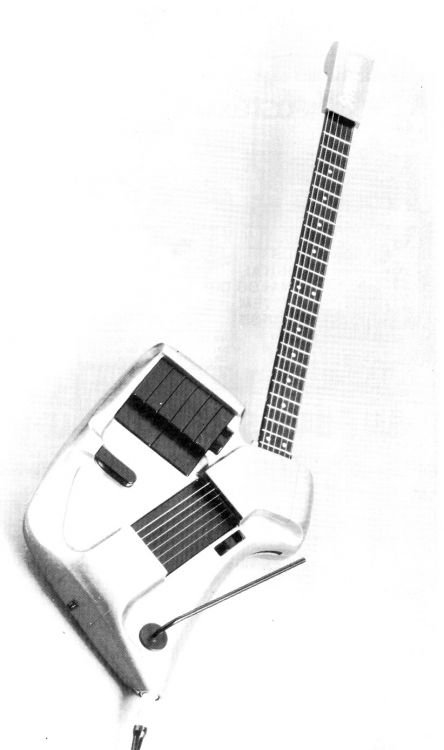
\includegraphics[scale=0.5]{Images/synthaxe.jpg}
    \caption{The \textit{SynthAxe}}
    \label{fig:synthaxe}
\end{figure}

The Yamaha EZ-EG \citep{yamaha_yamaha_2003} offers MIDI to the guitarist through the use of buttons. This is a good first step, but cannot offer aftertouch or pitch bends to the user, which limits its sonic capabilities. The Artihphon Instrument 1, is also making great steps in the right direction also incorporating elements of polyphonic aftertouch to the design, but cannot perform pitch bends on the neck of the guitar in the intuitive gesture that so many guitarists know and love. This project attempts to create a prototype that is not only capable of MPE pressure, but also of pitch bending. 



\subsection{Supporting Creativity and Flow in Studio Applications}
This study aims to develop the capacity of the augmented guitar to interact with digital instruments and DAWs in a musically pleasing and spontaneous way. As \cite{martelloni_percussive_2020} highlight, musicians can be wary of augmenting their performance with digital technologies, for fear of coming up short with respect to spontaneity and creativity.

This insight could either be framed in terms of how digital instruments are somehow inherently un-spontaneous and not conducive to supporting creativity; however, it could also be viewed as a design problem. This echoes the perspective of \cite{norman_design_2013}, where the burden of creating a compelling digital product is well within reach, but the burden to do so falls on the shoulders of the designer. Thus, the aim of the design is two-fold: to reduce the barriers to creativity that are experienced when interacting with technology, but also to further develop new and creatively useful ``contact points", developing on the research of \cite{lahdeoja_approach_2008}. Contact points are defined by \cite{lahdeoja_approach_2008} as a mapping of a physical gesture/object interaction with sound.

The way that we create music is becoming more digital and `in the box' \citep{nash_supporting_2012}. This means that the amount that musicians are interacting with their computers in a musical context is increasing, and therefore these perceived ``limitations" of digital technology need to be reduced. Since the technological capabilities of the computer are great, we might expect that it should also afford great creative opportunities. It would seem, however, that the limitation is in the \textit{design} of these new musical interfaces, not their technological prowess.